%solar_letters.tex

% solar_prod.tex
\documentclass[12pt]{article}
\usepackage{setspace}
\usepackage[margin=1in]{geometry}
\usepackage{mathtools}
\usepackage{natbib} %for citet and citep
\usepackage{syntonly}
\usepackage{esdiff} %for writing partial derivatives
\usepackage{url} %for inserting urls
\usepackage{placeins}
\usepackage{textcomp} 
\usepackage{amsmath}
\usepackage{graphicx}
\usepackage{booktabs}

\doublespacing % from package setspacs

 \title{Lease or Buy? Quality differences and asymmetric information in California solar panels}

 \date{\today}

 \author{Johannes Mauritzen\\ BI Norwegian Business School\\ Trondheim Campus \\Department of Accounting, Auditing and Business Analytics \\johannes.mauritzen@bi.no\\\url{http://jmaurit.github.io}}

 \begin{document}
  \begin{spacing}{1} %sets spacing to single for title page
 	\maketitle

 \begin{abstract}
  I provide one of few empirical case studies of asymmetric information of quality in a durable good. This study is unique in observing quality directly. I use data from approximately 1000 rooftop solar photovoltaic systems in California with 4 to 5 years of monthly production data. Using a Bayesian hierarchical model, I find evidence that leased systems show a higher level of quality than those bought out-right. 

%  JEL Codes: L15, Q42
 \end{abstract}

 % \thanks{*I would like to thank...}
 % 
  \end{spacing}

\section{Introduction}

The theoretical literature on information asymmetry of quality is well established \citep{akerlof_market_1970, chan_prices_1982,tirole_theory_1988}. The theory has in turn spawned a broad empirical literature, especially in the finance \citep{michaely_pricing_1994, petersen_benefits_1994,adams_liquidity_2009,dobbie_information_2013}, accounting \citep{healy_information_2001} and marketing literature \citep{kirmani_no_2000}. 

Empirical studies of information asymmetry in the market for durable goods are scarcer. A durable good can be seen as a one-time purchase that provides a stream of services. Thus, even if transaction data is available on the purchase of the durable good, quality is judged by the subsequent stream of services. The existing empirical literature on information asymmetry in durable goods often makes use of proxies for quality. In a study of information asymmetry in the used aircraft market, \citet{gilligan_lemons_2004} uses aircraft brands as a proxy. \citet{peterson_adverse_2014} and \citet{emons_market_2009} also use brand reputation as a proxy in studies of adverse selection in used cars. This approach does not capture the substantial individual variation in quality both within and between brands and categories. 

I present a case-study using data on roof-top solar photovoltaic systems where quality can be inferred directly through monthly production data. A testable implication of the theory of asymmetric information of quality is that in the presence of asymmetric information, poor quality goods will tend to push out high quality \citep{akerlof_market_1970, tirole_theory_1988}. I compare production over time between panels that are leased and sold-outright, which both theoretical and empirical studies suggest may differ with respect to the presence of information asymmetry \citep{johnson_leasing_2003,johnson_leasing_2010, johnson_role_2014,hendel_adverse_1997,gilligan_lemons_2004}. 

Photovoltaic systems that were sold outright are plausibly subject to substantial information asymmetry of quality. Homeowners and small business owners can not be expected to have the expertise to judge the quality of panels. Concerns about quality were likely extenuated by the introduction of panels from Chinese manufacturers that were nearly completely new to the US market in the time-frame studied and did not have established reputations. Anecdotally, panels from these new manufacturers varied greatly in quality.\footnote{\url{http://www.nytimes.com/2013/05/29/business/energy-environment/solar-powers-dark-side.html?pagewanted=all&_r=0
}}  

The market for rooftop solar panels can be expected to be vulnerable to adverse selection due to asymmetric information on quality. Solar panels are experience goods, where a consumer learns about quality through use. In particular, poor quality panels will tend to show a higher degradation of output over time. Even then, consumers may find it difficult to measure the degradation as it can happen gradually, over many years. 

More so, solar panel systems are expected to last at least 20 years, thus their purchase can be considered a one-shot investment. This eliminates repeat buying as a mechanism for ensuring quality. Warranties may also be a relatively weak assurance of quality in the market for solar panels as both contractors and manufacturers are relatively new, tend to be heavily indebted and have recently shown a tendency to go bankrupt. 

However, over the period from 2010 to 2014 many of the larger solar contractors moved to leasing solar power systems to homeowners. Shifting ownership to the large contractors that install and finance the solar systems could alleviate the information asymmetry, as these contractors can take steps such as testing panels and visiting manufacturing sites to ensure quality.

In this article, I compare production levels over time between systems that are leased and sold outright, while controlling for other observable factors that could affect production.

Testing for the degradation in production of nearly 1000 panels is problematic using traditional econometric models. The data has a grouped structure with many monthly observations for each solar panel. Traditional econometric models using maximum likelihood estimation can only approximately account for this structure, and inference from models with many fixed effects may be unreliable\citep{gelman_bayesian_2013}. I use a Bayesian hierarchical model estimated using Markov Chain Monte Carlo (MCMC) simulation techniques. The results of the Bayesian model provide evidence that solar panel systems that were leased tend to show less degradation over time than those that were sold outright.

\section{California Solar Initiative, Data and Empirical Model}

The data used in this study is from the California Solar Initiative (CSI). CSI gives incentives for installing solar panels systems in California. For most smaller systems the incentive was given in the form of an upfront payout based on the expected production of the system. Larger systems were required to accept a performance based incentive based on actual production over 5 years (60 months). From the beginning of the program in 2007 this was defined as those over 100kW, but was lowered to 50kW from January 2008 and 30kW from January 2010. Solar panel installations of all sizes have the option of getting an incentive based on actual performance. The data is openly available on the website of CSI.\footnote{\url{http://www.californiasolarstatistics.ca.gov/current_data_files/}}

Below are the key variables present in the CSI data:

\begin{itemize}
\item Installation date
\item Location: address, zip code, county
\item System capacity
\item Name of system owner, host, and contractor
\item Third party owner (leased)
\item Use of single or double axis trackers
\item Year of installation
\end{itemize}

I include only those installations that have been producing for at least 4 years (48 monthly observations), where the maximum number of observations is 60 months of production data. The data covers similar vintages of solar panels -- those that were installed from 2007 through 2009, and which continued to produce through 2013. I removed systems where production was reported to be higher than what would be theoretically possible from a solar power system with a given nameplate capacity. I also removed systems that reported 0 production in a period. This could also be an indication of quality if zero production indicates a malfunction in the system. However, it is not possible to identify which zero observations reflect malfunctions versus reporting issues. 

The data has a clear grouped structure. Individual production data are grouped by the different solar panel systems. Each system is then in turn grouped into categories of leased or host-owned. Seasonality must also be adequately accounted for as well as other factors such as geographic location, use of tracking and idiosyncratic variation between systems.

I fit a Bayesian multilevel regression model using Markov-Chain Monte Carlo (MCMC). Bayesian models are especially useful in estimating multi-level models with many parameters. In a multi-level model, lower-level parameters within a certain group are themselves modeled as coming from a distribution characterized by ``meta-parameters.'' The estimated group-level parameters are a weighted average of both the observations within the group as well as the full set of observations in the dataset -- the feature of multilevel models called partial pooling. Partial pooling also serves as a natural form of parameter shrinkage, eliminating the need for corrections for multiple comparisons in inference \citep{gelman_data_2006}. 

For estimation we use the Stan Bayesian programming language \citep{stan_development_team_stan_2014}, which uses Hamiltonian MCMC and a No U-Turn Sampler (NUTS) to estimate a joint posterior distribution of the probability model. \citet{kruschke_doing_2014} provides an accessible explanation of the Hamiltonian MCMC algorithm, while more detailed technical descriptions are provided by \citet{gelman_bayesian_2013} and the Stan reference manual \citep{stan_development_team_stan_2014}.

Figure \ref{solar_prod_bayes_diag} shows the structure of the model. Starting from the bottom, the individual production data are log transformed and modeled as having a Cauchy distribution with mean $\hat{y}$ and variance $\sigma$. $\sigma$ is in turn given a half-Cauchy prior. 

The use of the Cauchy and half-Cauchy distribution reflects that a large-in-magnitude effect of around 5 or greater on the logit scale is highly unlikely in logistic regressions where all non-binary data has been transformed to have mean zero and standard deviation 1. The Cauchy distribution will also give answers even under complete separation, and avoids computational problems inherent in assigning completely non-informative priors in multilevel models \citep{gelman_weakly_2008}.

Going up a level, $\hat{y}$ is modeled as having random group-level intercepts $\beta_{0,j}$, where j represents the j-th of $J$ solar panel system. The $\beta_{0,j}$'s are in turn modeled as function of system size, county, whether solar trackers are used, and a random effects term $re_j^0$. 

In a similar manner the J $B_j$ coefficients are modeled as a function of whether the system is leased, $\mu_{lease}^1$, the host sector of the installation, the county, use of tracking, installation year and a random effects term $re^1_j$.  The question of interest -- whether leased solar systems display a lower degree of degradation over time than those sold outright -- can then be expressed as the distribution of the difference of the $\mu_{lease}$ parameters: $\mu_{lease=1} - \mu_{lease=0}$.

Finally, to take into account the seasonality of the monthly data, random effects for each of the 12 months are estimated with a $Cauchy(0,4)$ prior on each parameter. The remaining hyper-parameters are given Cauchy or half-Cauchy priors. 

\begin{figure}
	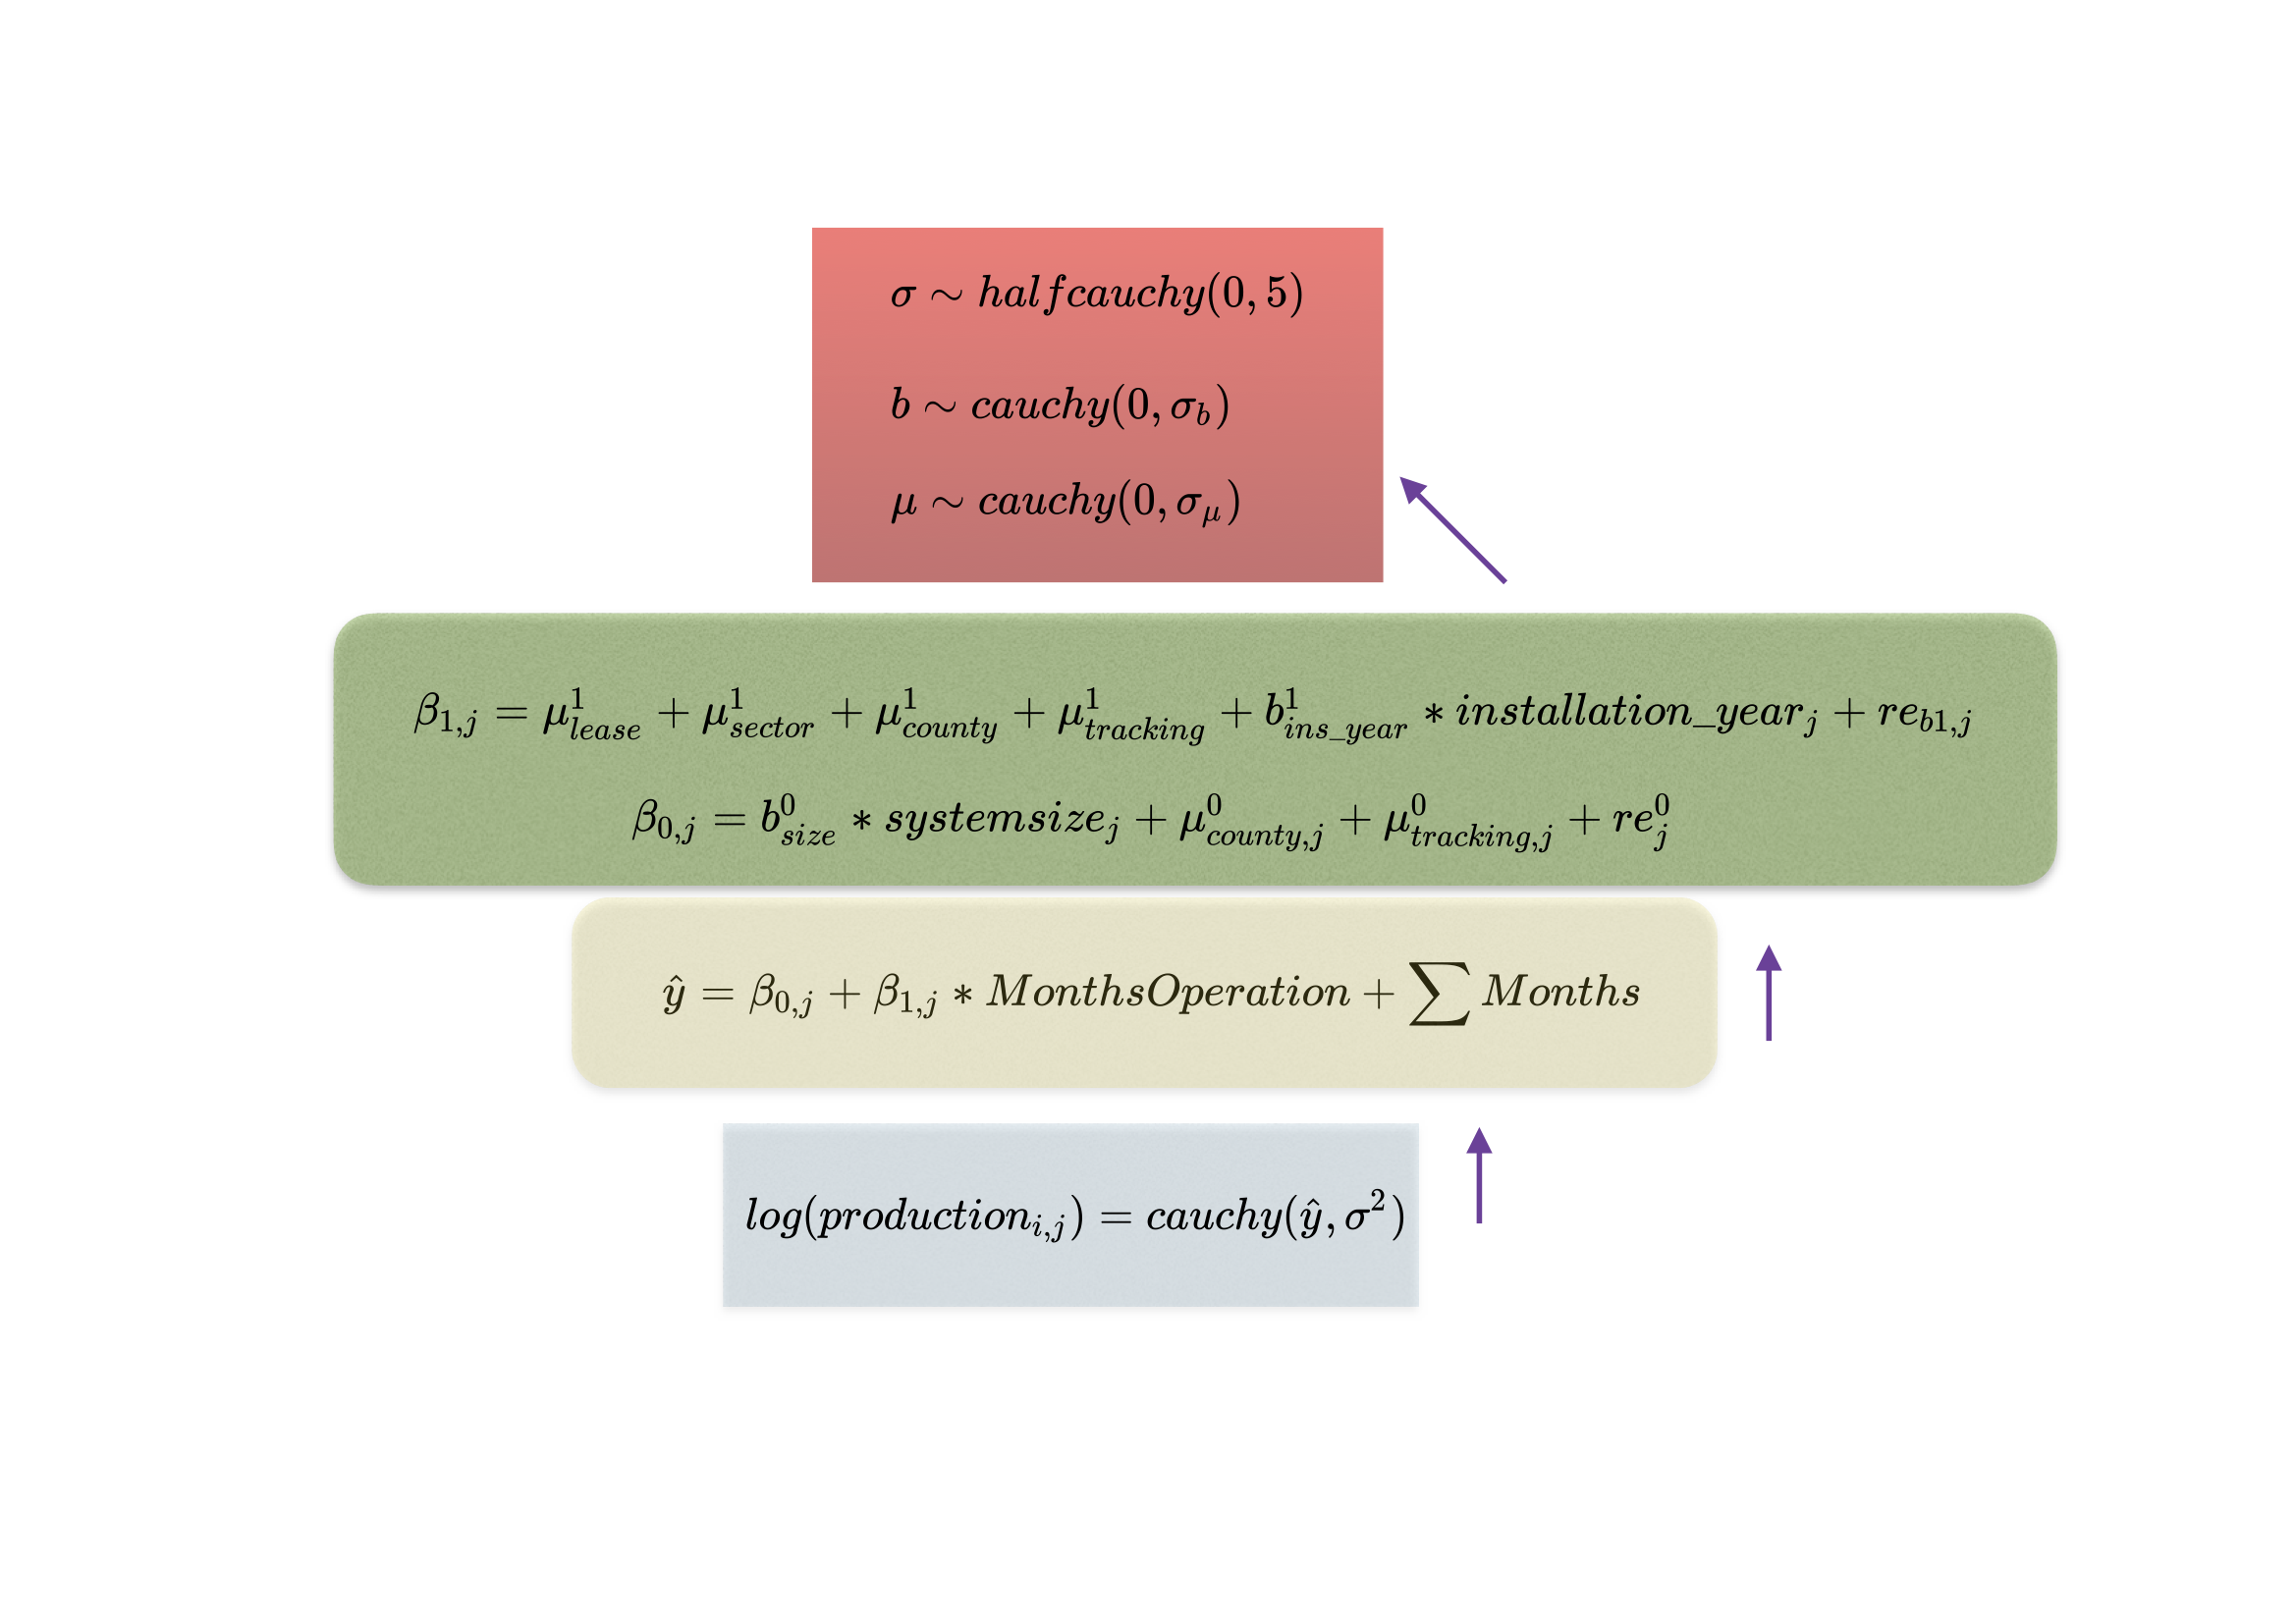
\includegraphics[width=1\textwidth]{figures/solar_prod_bayes_diag.png}
	\caption{The data and the research question combined suggest a hierarchical Bayesian model. The figure shows the structure of the model. Production data is grouped by individual solar panel systems.}
	\label{solar_prod_bayes_diag}
\end{figure}

\section{Results}

Summary statistics for the posterior distributions of the main parameters of the model are shown in table \ref{table_results}. The parameters of interest are $\mu_{lease=1}$ and $\mu_{lease=0}$, which are the average slope of production over time in, respectively, systems that were sold outright and systems that were leased. These coefficients should be interpreted for a marginal change of 1 standard deviation change in time. 

\begin{table}
\footnotesize
\resizebox{12cm}{!} {
\begin{tabular}{lrrrr}
\toprule
{} &  2.5\%&   97.5\% &   mean &  median \\
params           &          &          &         &          \\
\midrule
apr              &   0.1452 &  -0.0838 &  0.0069 &  -0.0013 \\
aug              &   0.2065 &  -0.0223 &  0.0681 &   0.0594 \\
dec              &  -0.1005 &  -0.3295 & -0.2386 &  -0.2471 \\
feb              &  -0.1037 &  -0.3346 & -0.2437 &  -0.2523 \\
jan              &  -0.1935 &  -0.4234 & -0.3319 &  -0.3404 \\
jul              &   0.2364 &   0.0058 &  0.0968 &   0.0886 \\
jun              &   0.2584 &   0.0282 &  0.1191 &   0.1105 \\
mar              &  -0.0257 &  -0.2535 & -0.1631 &  -0.1717 \\
may              &   0.2067 &  -0.0225 &  0.0687 &   0.0602 \\
nov              &   0.0546 &  -0.1748 & -0.0839 &  -0.0923 \\
oct              &   0.1256 &  -0.1034 & -0.0124 &  -0.0211 \\
sep              &   0.2094 &  -0.0205 &  0.0704 &   0.0619 \\
mu1\_commercial   &   0.0014 &  -0.0041 & -0.0007 &  -0.0005 \\
mu1\_government   &   0.0035 &  -0.0026 &  0.0004 &   0.0002 \\
mu1\_non\_profit   &   0.0018 &  -0.0057 & -0.0008 &  -0.0003 \\
mu1\_not\_tracking &   0.0044 &  -0.0074 & -0.0016 &  -0.0009 \\
mu1\_residential  &   0.0039 &  -0.0023 &  0.0005 &   0.0003 \\
mu1\_tracking     &   0.0039 &  -0.0092 & -0.0021 &  -0.0014 \\
mu\_lease         &  -0.0001 &  -0.0115 & -0.0045 &  -0.0042 \\
mu\_own           &  -0.0001 &  -0.0125 & -0.0054 &  -0.0054 \\
beta0\_size       &   0.7501 &   0.6948 &  0.7173 &   0.7141 \\
beta1\_ins\_year   &  -0.0007 &  -0.0032 & -0.0020 &  -0.0020 \\
beta1\_size       &  51.1251 & -45.7583 &  0.1312 &   0.0594 \\
sigma            &   0.0295 &   0.0287 &  0.0291 &   0.0291 \\
\bottomrule
\end{tabular}
}
\label{table_results}
\caption{Summary statistics of the distributions over the main parameters in the model. Confidence intervals are estimated as quantiles at 2.5 and 97.5 percent of the estimated posterior distribution of the parameters.}
\end{table}

In figure \ref{diff_lease}, I show a histogram of the posterior of the difference between the two parameters, $\mu_{lease=1} - \mu_{lease=0}$. A direct interpretation is then that there is an approximately 80\% probability that on average solar power systems that are sold outright have a higher rate of degradation than those that are leased. 

\begin{figure}
	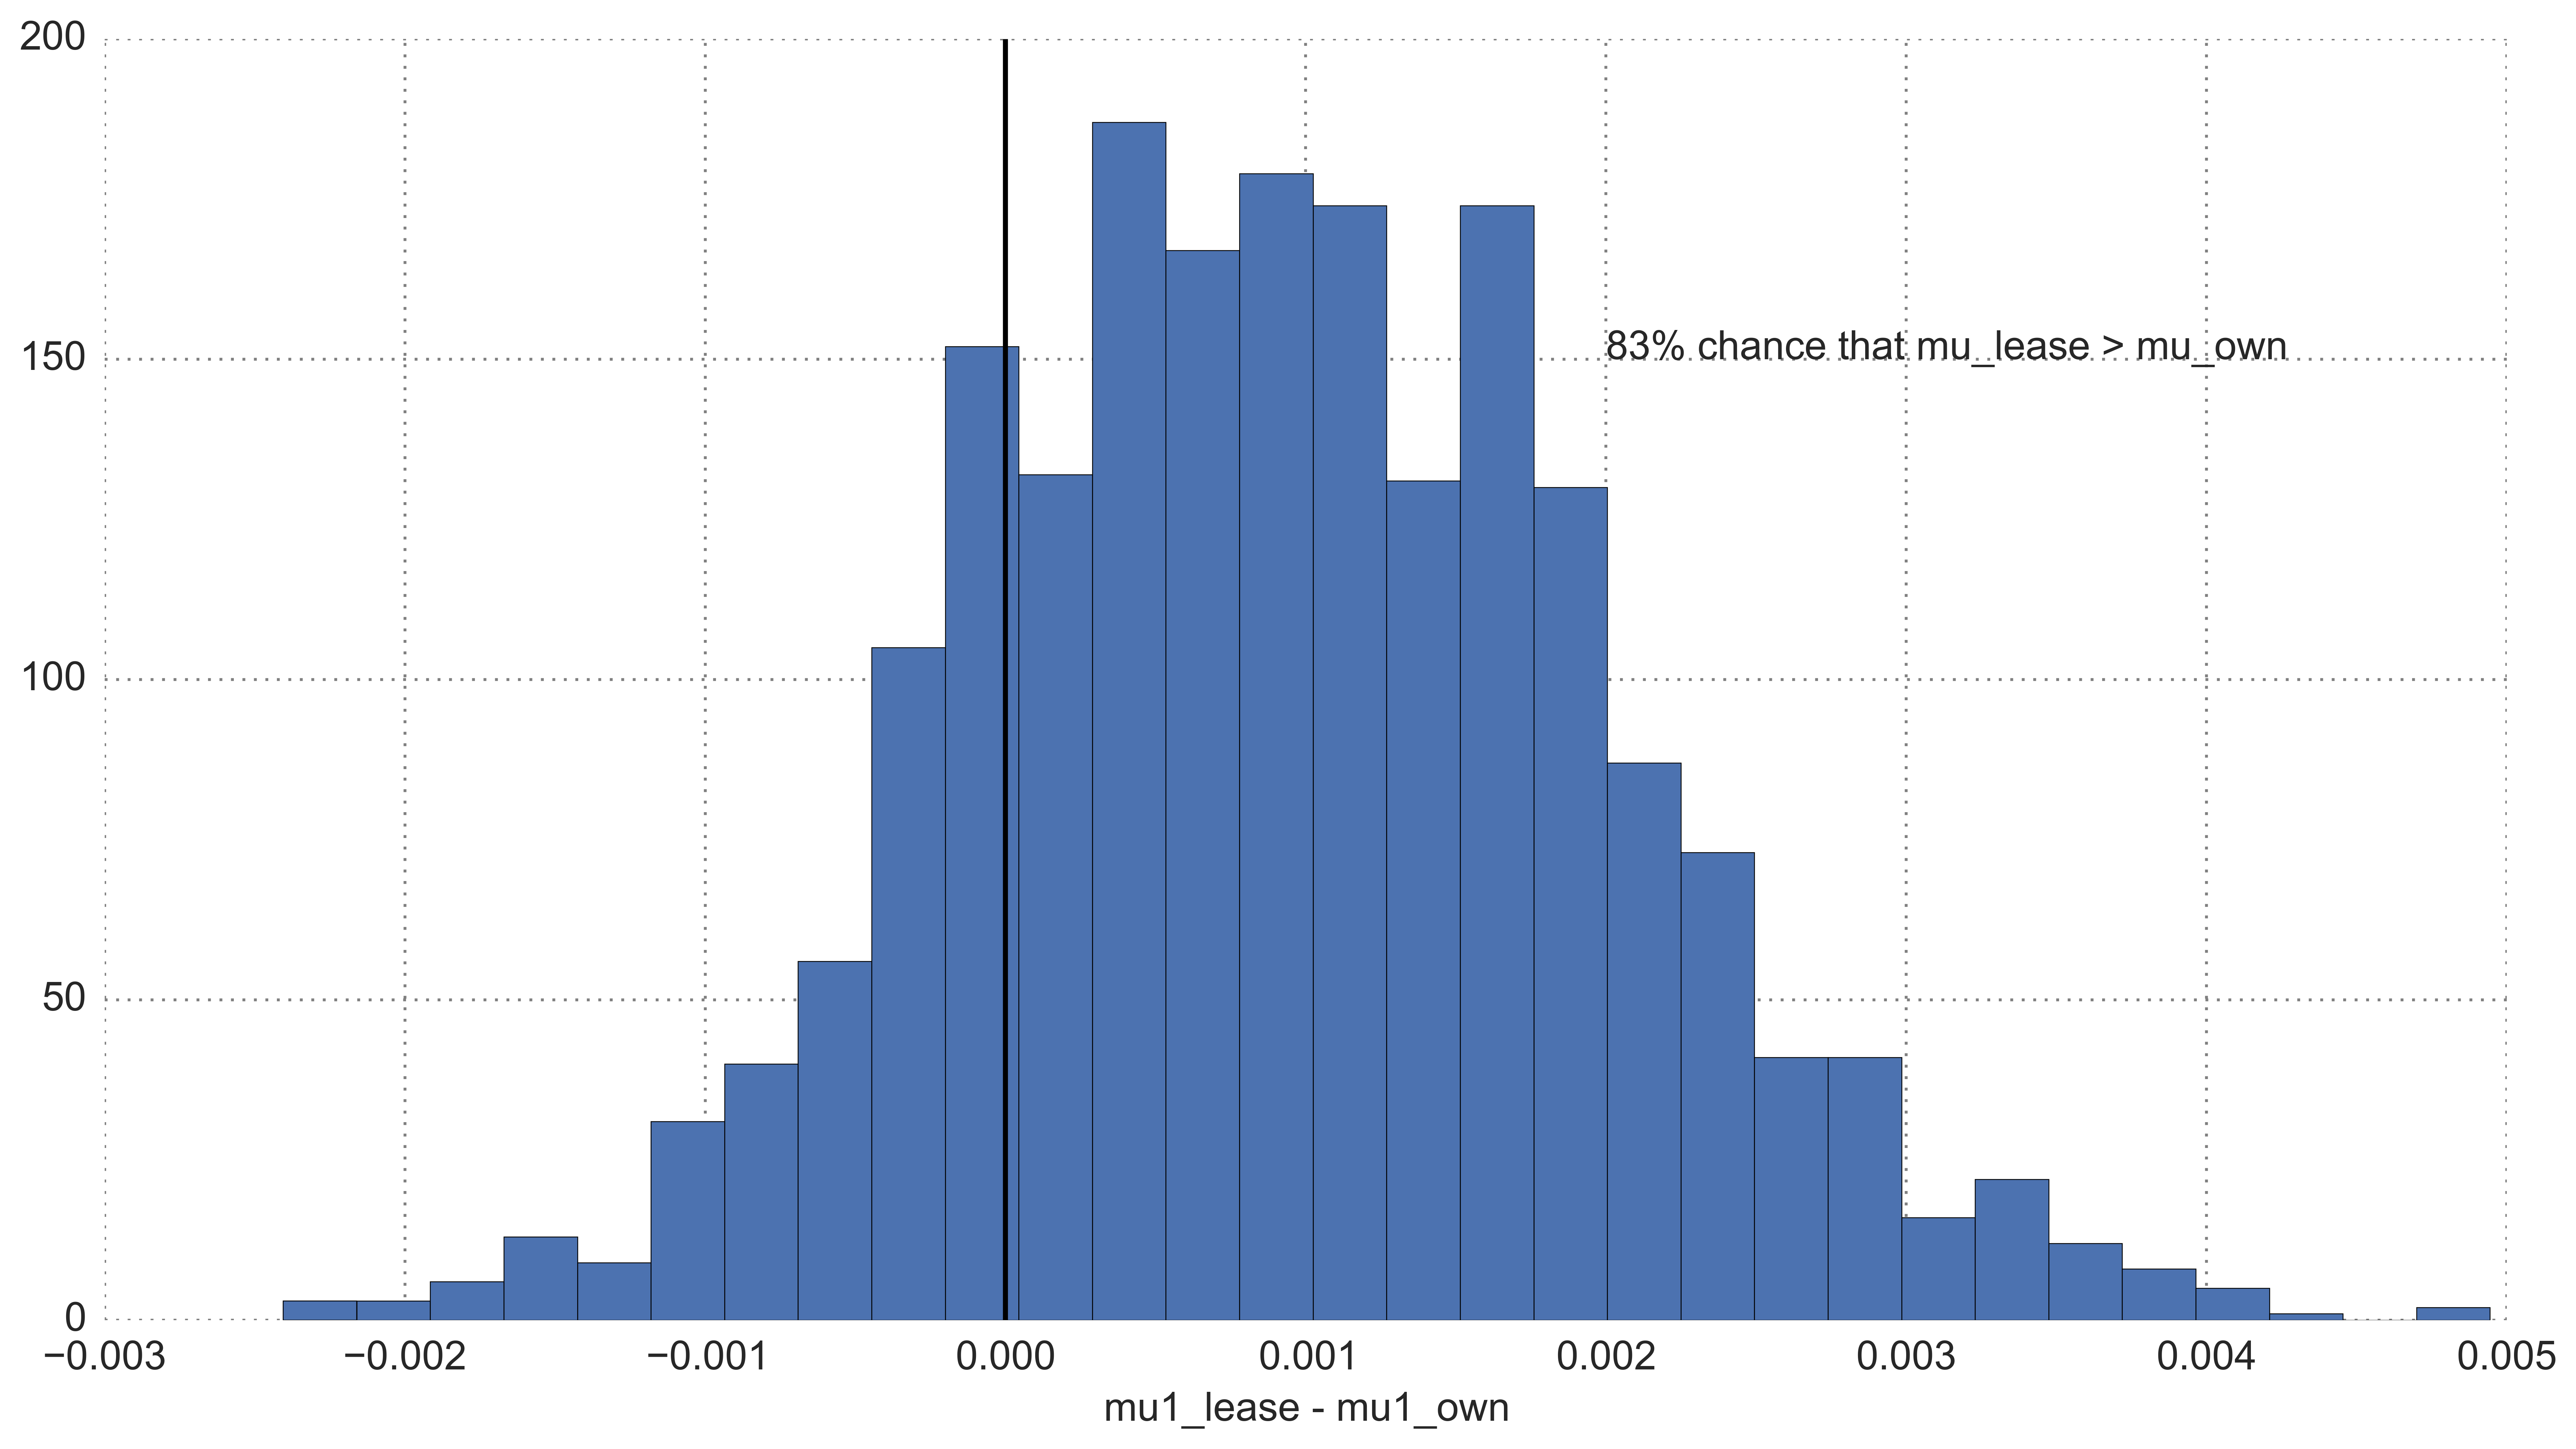
\includegraphics[width=1\textwidth]{figures/diff_lease.png}
	\caption{The figure shows the distribution of the difference of $\mu_{lease=1}$ and $\mu_{lease=0}$. The black vertical line is placed at zero. The distribution of the difference of the two parameters suggests that leased panels had about a 80\% chance of being higher quality than those sold outright, as measured by the slope of production over time.}
	\label{diff_lease}
\end{figure}

The magnitude of the effect can best be seen by plotting average predicted values over time, which are shown for systems that are leased and sold-outright in figure \ref{predicted_deg}. The solid lines represent the median value of the posterior distribution on the $\mu_{lease=1}$ and $\mu_{lease=0}$ parameters, where the light lines represent random draws from the respective posterior distributions. The model results suggest that a leased solar panel system will on average experience degradation of about 6\% after 20 years while those owned outright experience on average 5\% of degradation. However, as the figure makes clear, the average values hide significant variation in the overall distribution.

\begin{figure}
	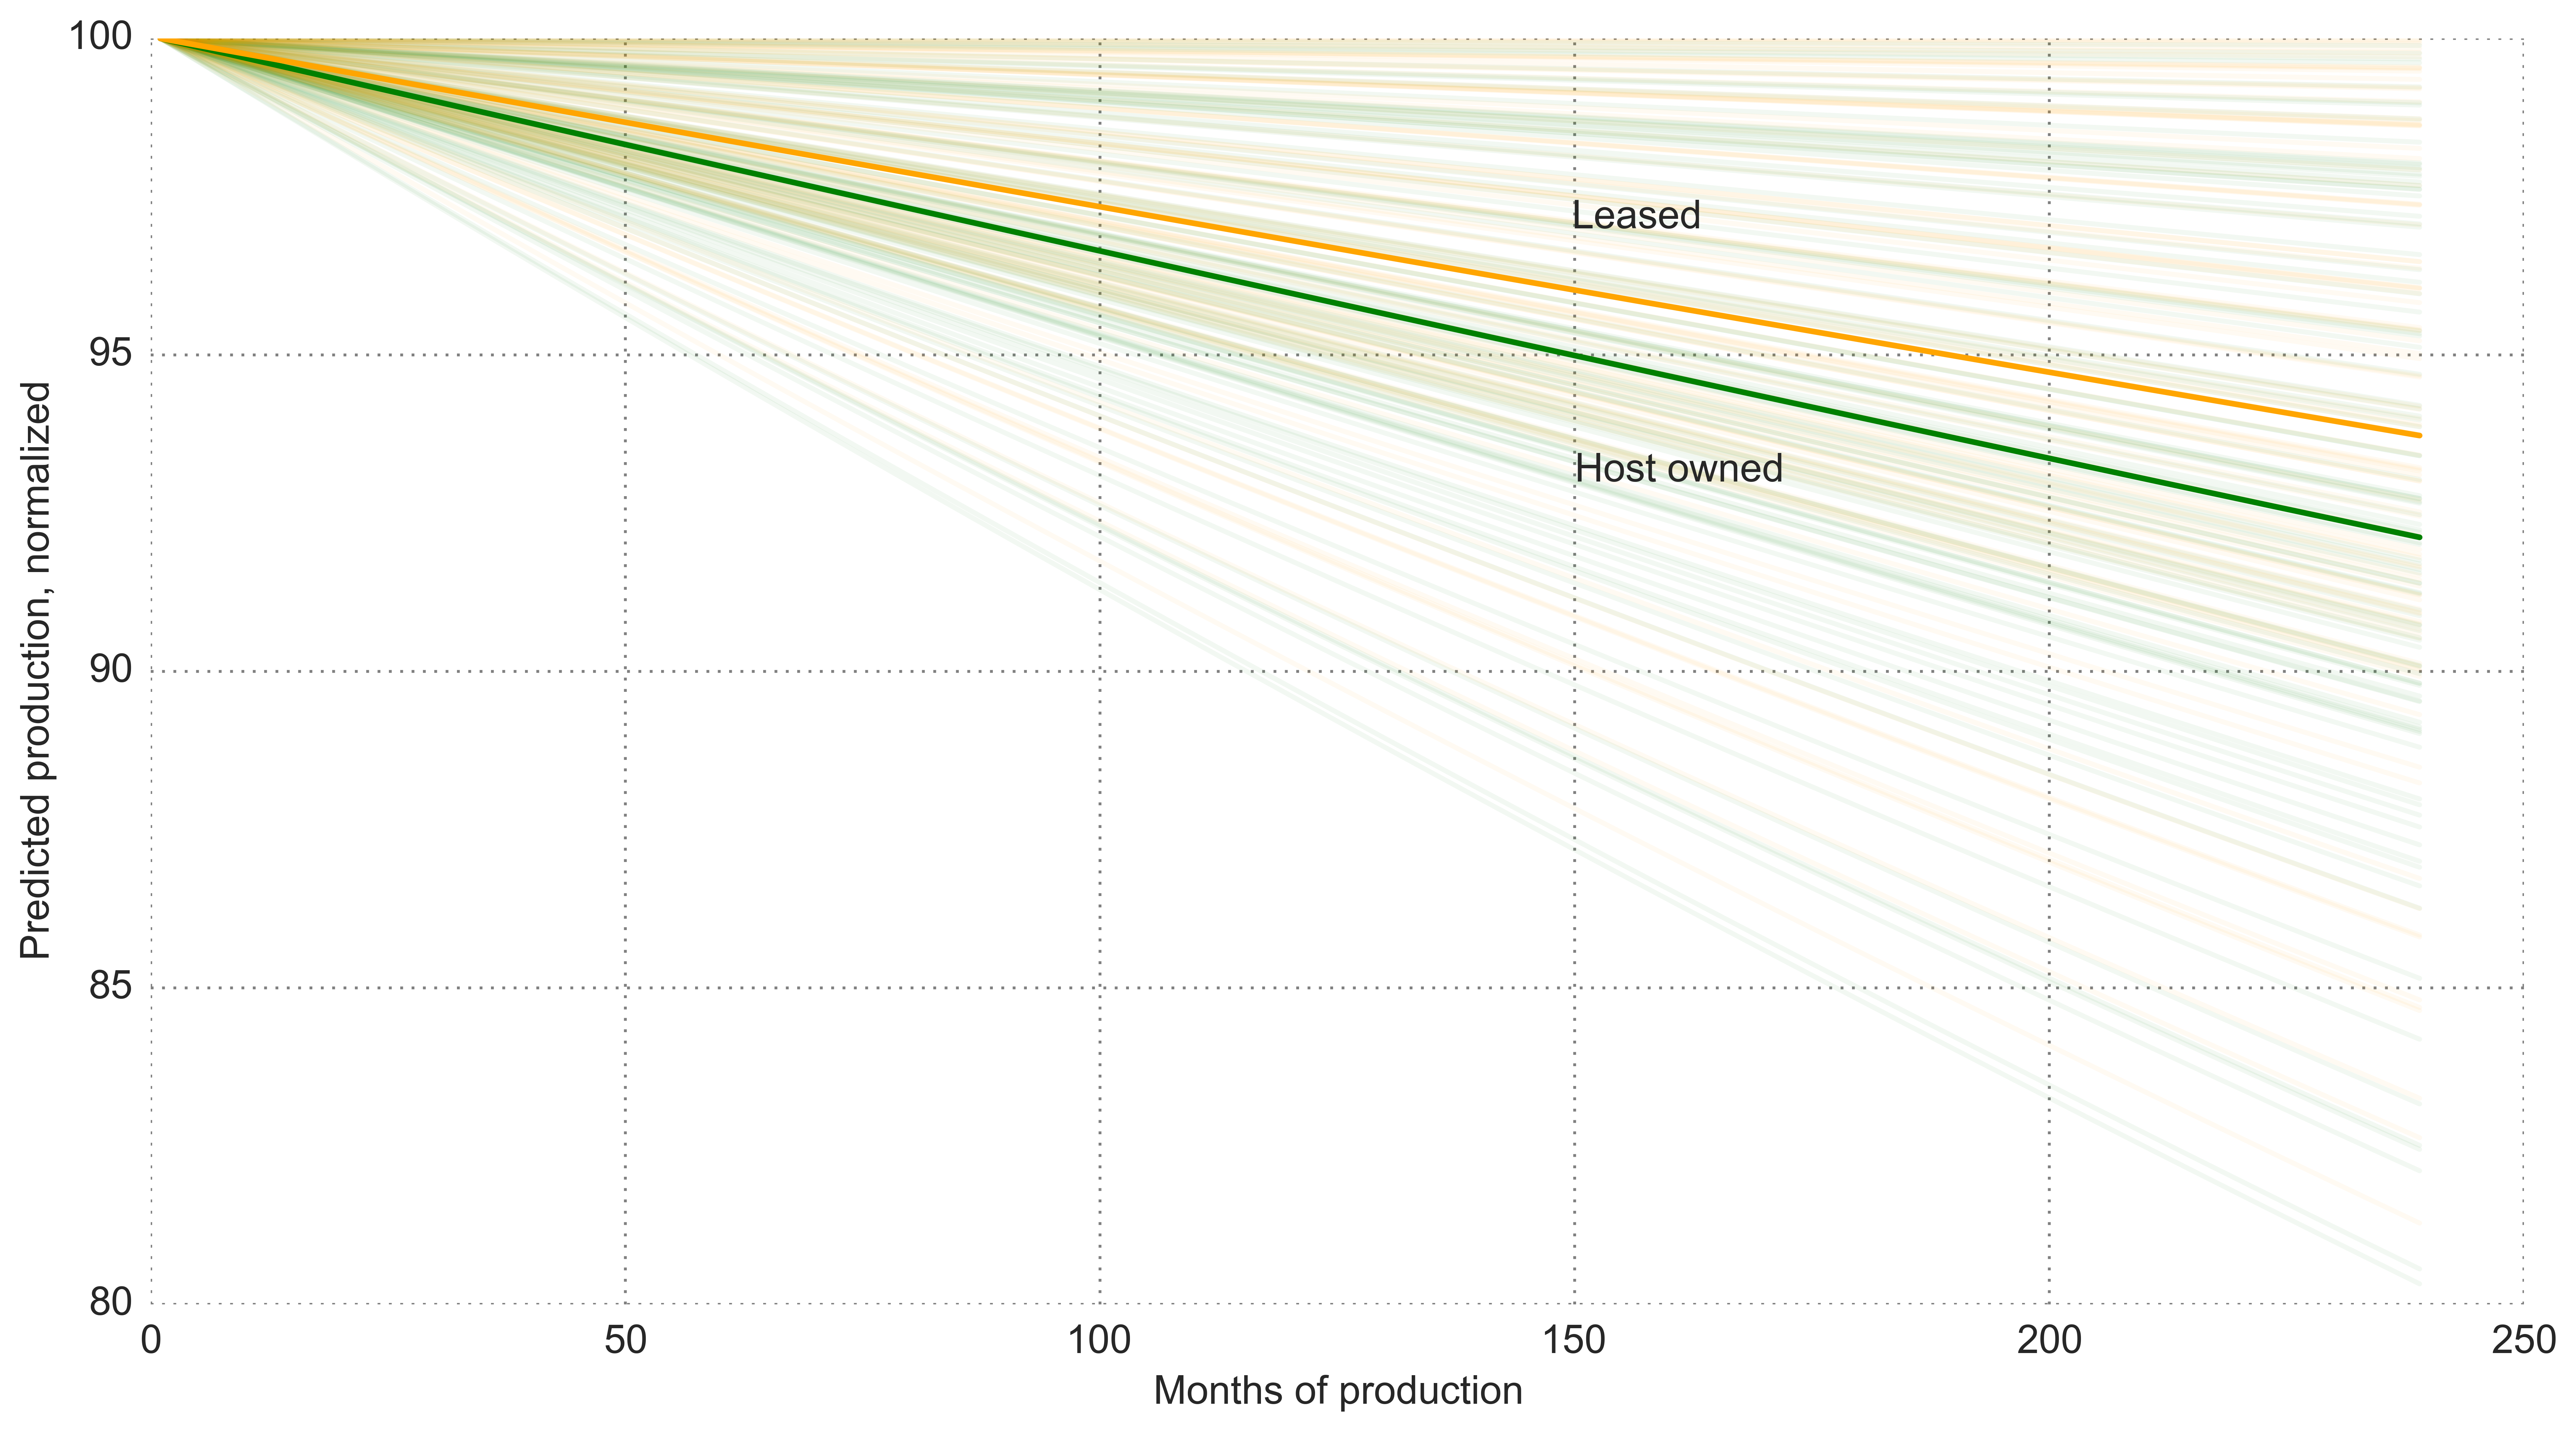
\includegraphics[width=1\textwidth]{figures/predicted_deg.png}
	\caption{The figure shows the average predicted values of degradation over time of solar panel systems that are leased and sold out-right. The solid lines represent the mean value of the posterior where the lighter lines represent random draws from the posterior distribution.}
	\label{predicted_deg}
\end{figure}

\section{Conclusion}
The theoretical literature on information asymmetry and quality is established and deep. The empirical literature for consumer durable investments is, however, sparse, reflecting the difficulty of getting reliable data on purchases and long-term reliability. This article provides one of few case studies that both identifies a market that could be expected to have issues of information asymmetry of quality, and provides a direct empirical test of the implications from the theoretical literature.  

The use of Bayesian MCMC simulation techniques in this article also provides an illustrative example of the use and usefulness of a powerful emerging tool-set. The Bayesian frameworks and recently developed software such as Stan provide major practical and theoretical advantages over many traditional econometric methods.

\begin{spacing}{1}
\bibliographystyle{plainnat}
\bibliography{solar_prod}

\FloatBarrier

\end{spacing}
\end{document}
